\section{Problem Definition and DA-HELLO Design}
\label{sec:design}
A HELLO is useful only if it changes what a receiver does, yet a sender cannot see its receivers' state. This section states that as a scheduling problem and then gives DA-HELLO, a causal heuristic that approximates it from the sender's own history. Only the scheduler is described here; the host routers and the state carriers are those of Section~\ref{sec:prelim}.

\subsection{Problem Definition}
\label{sec:problem}
Let $U_{j,k}\in\{0,1\}$ indicate that node $s_j$ requests a HELLO at decision epoch $k$ of period $\Delta t$. A request can be queued, delayed, or dropped by the MAC, and a transmitted HELLO can collide or fall below the decoding threshold, so a request neither guarantees a transmission nor refreshes any particular receiver. Between frames, every receiver holds a zero-order copy of the advertised vector $\xi_j$, while the true attributes keep evolving.

Not every change matters to a receiver. Let $m_j$ be an advertisement of $s_j$ and $\mathcal{U}_h(X_i^h,m_j,y_{ij})$ the host's processing of its successful reception at $s_i$, where $X^h_i$ holds the held records and learning state and $y_{ij}$ is the reception metadata. For a diagnostic recipient set $\mathcal{C}_j$, define
\begin{multline}
D_j=\mathbf{1}\big\{\exists\, i\in\mathcal{C}_j:\ \mathcal{R}_h(X_i^{h,+};\kappa_i)\neq \mathcal{R}_h(X_i^h(t^-);\kappa_i)\big\},\\
X_i^{h,+}=\mathcal{U}_h\big(X_i^h(t^-),m_j,y_{ij}\big),
\label{eq:relevance}
\end{multline}
that is, the advertisement matters if some receiver's forwarding output $\mathcal{R}_h$ for a packet context $\kappa_i$ would change. Missing and expired records are included in the hypothetical reception, so a first contact is relevant because a node that has never recorded $s_j$ cannot rank it. Candidacy changes and sign changes of the score gap $g_{ijc}=\sigma_i(j)-\sigma_i(c)$ to a co-candidate $s_c$ are the two ways the output can change. $D_j$ is a receiver-specific offline \emph{diagnostic}: it needs the receivers' state, so it cannot be an input to a node, and it was not measured in our campaign. An update can also be useful later when the immediate output is unchanged, and a changed output can be harmful, so $D_j$ does not define an optimal schedule.

Let $B(\pi)$ be the control bytes sent under a HELLO policy $\pi$ and $\mathrm{PDR}(\pi)$ the delivery ratio of a fixed host router. With a reference policy $\pi_{\mathrm{ref}}$ and a non-inferiority margin $\delta_P$, the \emph{host-parametric HELLO scheduling problem} is
\begin{equation}
\min_{\pi}\ \mathbb{E}\,[B(\pi)]\quad\text{s.t.}\quad \mathbb{E}\,[\mathrm{PDR}(\pi)]\ \ge\ \mathbb{E}\,[\mathrm{PDR}(\pi_{\mathrm{ref}})]-\delta_P,
\label{eq:problem}
\end{equation}
over causal policies $U_{j,k}=\pi_j(\mathcal{H}_j(t_k),Z_{j,k})$ that depend only on the node's own history $\mathcal{H}_j$ and local randomness $Z_{j,k}$. The problem involves the host only through the candidate set $\mathcal{I}^h$ and the score $\sigma_i$, not through its learning rule, so any host that exposes them poses the same problem. Energy enters through $B$ and through the delivery count in (\ref{eq:runmetrics}). DA-HELLO is an experimentally assessed heuristic for (\ref{eq:problem}), not an optimiser, and sending a HELLO exactly when $D_j=1$ is not claimed to be optimal. The reference in our primary HELLO-only comparison is the 120\,s periodic policy, not a policy selected for its outcome.

\subsection{Design Overview}
\label{sec:overview}
DA-HELLO follows three principles. It is \emph{host-parametric}: it uses the host only through the candidate set, the score, and a broadcast primitive. It is \emph{causal}: every input is the node's own state, a decoded frame, or a held record. And it works on \emph{requests}: the scheduler decides when to ask for a HELLO, and the MAC decides when, and whether, it is sent. Fig.~\ref{fig:flow} shows the structure. All policies in Section~\ref{sec:eval}, including the no-HELLO arm, start from the same join announcement: each node sends one HELLO after a random delay, and the sink broadcasts a beacon at a fixed period throughout. After joining, DA-HELLO raises a request on four conditions.

\begin{figure*}[t]
\centering
% t183: Ali-supplied Fig. 3 (replaces TikZ fig_flow). Do not hand-edit the PDF.
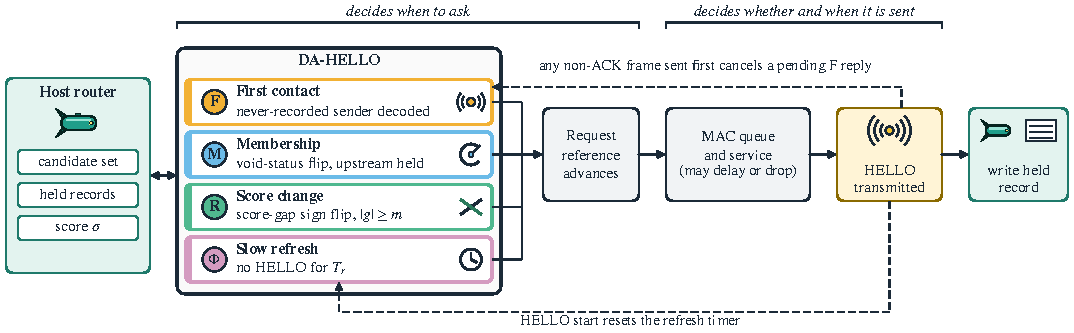
\includegraphics[width=\textwidth]{fig3_flow}

\caption{Structure of DA-HELLO beside a host router. Four conditions on the node's own history raise a request; the request advances a sender reference, passes through the MAC, and a HELLO that is decoded writes the receivers' held records. A pending first-contact reply is cancelled if the node sends any non-ACK frame first.}
\label{fig:flow}
\end{figure*}

\subsection{Trigger Conditions}
\label{sec:policy}
At epoch $k$, a node requests a HELLO if
\begin{equation}
U_{j,k}=\mathbf{1}\{F_j\vee M_{j,k}\vee R_{j,k}\vee \Phi_{j,k}\},
\label{eq:request}
\end{equation}
where the conditions are evaluated in the order $M$, $R$, $\Phi$ and at most one request is raised per epoch. One HELLO serves all pending requests of the node.

\emph{First contact ($F$).} When $s_j$ decodes a frame from a sender $s_x$ that it has never recorded, it schedules a reply after a random delay $u\sim\mathcal{U}[0,u_{\max}]$, with a minimum separation $g_{\min}$ between reply releases. Several discoveries can share one pending reply, and the separation is a release-side limit, not a bound on the spacing of physical transmissions after MAC queueing. The test uses the node's own record of $s_x$ before the frame is written. That record is created by the first decoded state-bearing frame and is never cleared, so ``new'' means never recorded, not recorded and since expired. The reply is cancelled if the node begins any non-ACK transmission before it fires.

\emph{Membership ($M$).} Let $v_j(t)=\mathbf{1}\{\mathcal{I}^h_j(t)=\emptyset\}$ be the void indicator of $s_j$ and $\mathcal{A}_j(t)$ the approximate upstream-interest set formed from its fresh records and held depths. Then
\begin{equation}
M_{j,k}=\mathbf{1}\{v_j(t_k)\neq v_j^{\mathrm{ref}}\ \wedge\ \mathcal{A}_j(t_k)\neq\emptyset\},
\label{eq:membership}
\end{equation}
where $v_j^{\mathrm{ref}}$ is the void status at the last request. This is a void-status heuristic, not a detector for every change in a receiver's candidate set: a receiver that $s_j$ has never heard can be absent from $\mathcal{A}_j$.

\emph{Score change ($R$).} Let $g^{\mathrm{ref}}_{jc}$ and $g^{\mathrm{now}}_{jc}$ be the score gap between $s_j$ and a held co-candidate $s_c$ computed with the score at the last request and with the current score. A non-void node raises
\begin{multline}
R_{j,k}=\mathbf{1}\{v_j(t_k)=0\ \wedge\ t_k\ge\tau_j\ \wedge\\
\exists\, c:\ g^{\mathrm{ref}}_{jc}\,g^{\mathrm{now}}_{jc}<0,\ |g^{\mathrm{now}}_{jc}|\ge m\},
\label{eq:rank}
\end{multline}
with margin $m$ and hold deadline $\tau_j$. A void event resets the interval $I_j$ to $I_{\min}$; each accepted rank event doubles it up to $I_{\max}=I_{\min}2^{d}$ with $d$ doublings and sets $\tau_j=t_k+I_j$. This back-off acts on rank requests only; it is distinct from MAC contention back-off and from Trickle's consistency-based suppression.

\emph{Slow refresh ($\Phi$).} With period $T_r$ and the time $t^{\mathrm{last}}_j$ of the node's last HELLO,
\begin{equation}
\Phi_{j,k}=\mathbf{1}\{T_r<\infty\ \wedge\ t_k-t^{\mathrm{last}}_j\ge T_r\},
\label{eq:refresh}
\end{equation}
and $T_r=\infty$ disables it.

\subsection{Algorithm}
\label{sec:algo}
Algorithm~\ref{alg:da} gives the receive handler and the per-epoch procedure.

\begin{algorithm}[t]
\caption{DA-HELLO at node $s_j$}
\label{alg:da}
\begin{algorithmic}[1]
\Require held records; references $g^{\mathrm{ref}}_{jc}$, $v^{\mathrm{ref}}_j$, $t^{\mathrm{last}}_j$, $\tau_j$; parameters $(m,I_{\min},d,T_r,u_{\max},g_{\min})$
\Statex \textbf{On decode of a frame from $s_x$ (before the record is written):}
\If{$s_x$ never recorded by $s_j$}
  \State schedule or merge a first-contact reply after $u\sim\mathcal{U}[0,u_{\max}]$, not earlier than $g_{\min}$ after the previous reply release
\EndIf
\Statex \textbf{On start of any non-ACK transmission of $s_j$:}
\State cancel the pending first-contact reply
\Statex \textbf{At each epoch $t_k$:}
\State $U\gets 0$
\If{$M_{j,k}=1$}
  \State $U\gets 1$; $I_j\gets I_{\min}$ \Comment{membership}
\ElsIf{$R_{j,k}=1$}
  \State $U\gets 1$; $I_j\gets\min(2I_j,\,I_{\min}2^{d})$; $\tau_j\gets t_k+I_j$ \Comment{score change}
\ElsIf{$\Phi_{j,k}=1$}
  \State $U\gets 1$ \Comment{slow refresh}
\EndIf
\If{$U=1$}
  \State update $g^{\mathrm{ref}}_{jc}$ and $v^{\mathrm{ref}}_j$ from the current state; request a HELLO
\EndIf
\end{algorithmic}
\end{algorithm}

\subsection{Host Instantiation}
\label{sec:hosts}
The score $\sigma$ is host-specific, and each surrogate below is a local approximation of the order that neighbours compute. For MARV it is
\begin{equation}
\sigma^{\mathrm{M}}_j=-w_E\Big(1-\frac{e_j}{E_0}\Big)-w_D\frac{z_j}{R_s}+\gamma(\lambda_1-\lambda_2)V_j,
\label{eq:marv_score}
\end{equation}
with the host's energy and depth weights $w_E,w_D$, normalisation energy $E_0$, range scale $R_s$, and value $V_j$. The current self depth is used in both the reference and the current score, and competitor values come from the node's own held records, with the fixed sink depth taken as an a-priori constant. For QELAR it is
\begin{equation}
\sigma^{\mathrm{Q}}_j=\frac{e_j}{E_0}+c_n\,n_j+\gamma\,V_j,
\label{eq:qelar_score}
\end{equation}
with $n_j$ the size of the candidate set and $V_j$ the node's own value; the peer score uses the held energy of $s_c$ and sets its count and value to zero. This is a heuristic proxy for the stored Q-ordering of neighbours, not an exact reconstruction, and the asymmetric substitution can influence which crossings occur. Because the rank test rests on a surrogate, a rank request is evidence for a trigger condition, not proof that a remote forwarding decision changed. The constants $c_n$ and $\gamma$ are the host's own.

\subsection{Request Semantics of the Evaluated Implementation}
\label{sec:semantics}
Four details matter for reading the results. First, the medium samples the sender's advertised fields into a frame at the start of an actual control transmission, and receivers apply those sampled values after decoding, so a later sender value is never substituted at decode time. Second, the references advance when a request is accepted by the scheduler, before the MAC serves it, so a reference is the last requested value, not necessarily the last transmitted one; MARV also advances its sender reference on a data transmission, including in the HELLO-only variant where receivers ignore the attributes of data frames. Third, the cancellation rule is kind-based: any non-ACK transmission cancels a pending reply, whether or not it carried the fields the reply would have supplied, and in the HELLO-only variants this includes stripped data frames. Fourth, the refresh timer is reset at the start of a HELLO transmission in MARV, but at the request and at control transmissions in QELAR, so a configured $T_r$ is not a bound on the age of a receiver's record. Counters of membership, rank, refresh, and reply-release \emph{requests} are therefore never summed as HELLOs; physical control traffic is counted from the medium's frame-start tally. A stricter field-aware controller would change the policy, and its results would not follow from those reported here.

\subsection{Properties and Scope}
\label{sec:scope}
The per-epoch cost is $O(|\mathcal{N}_j|)$ in the number of held neighbours. Beyond the host primitives of Section~\ref{sec:prelim}, DA-HELLO adds a few scalars of state per node ($g^{\mathrm{ref}}_{jc}$, $v^{\mathrm{ref}}_j$, $t^{\mathrm{last}}_j$, $\tau_j$) and a pending-reply timer. It is host-parametric in the sense that it needs only $\mathcal{I}^h$, $\sigma$, and a broadcast primitive. It is not self-configuring: the parameters differ by host class and state carrier (Section~\ref{sec:eval}).
